\subsection{Account}

Account-klassen sørger for at vedligeholde spillernes konti. Den opretter accounts med en balance, og hver spiller får på den måde tildelt et account herfra.

Man kan trække penge fra hver spillers account med withdraw() metoden. Den tager spillerens account og trækker en mængde fra.
\begin{figure}[H]
    \centering
    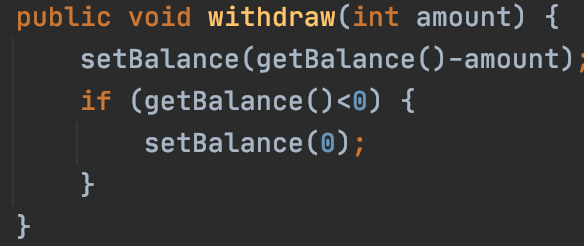
\includegraphics[width=\textwidth]{sources/7_implementering/Withdraw.PNG}
    \caption{Withdraw metode}
    \label{fig:accWithdraw}
\end{figure}
Ligeledes har vi en deposit metode, som overfører en pengesum til en spiller. Dette sker bl.a. når en spiller krydser start, eller modtager husleje af en anden spiller.
\begin{figure}[H]
    \centering
    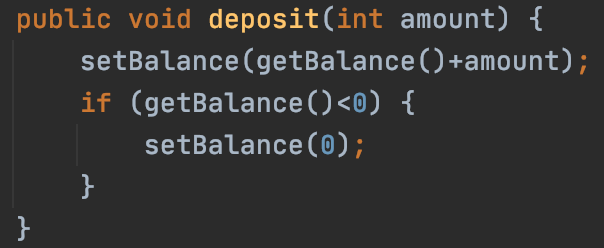
\includegraphics[width=\textwidth]{sources/7_implementering/Account Deposit.png}
    \caption{Account Deposit metode}
    \label{fig:accDeposit}
\end{figure}
efterfølgende ligger getStartingBalance, hvor spillere modtager 30.000 ved spillets start hver især. 
Derefter har vi crossStartMoney, som gør brug af deposit til at give spillere 4.000, når de krydser start-feltet.
\begin{figure}[H]
    \centering
    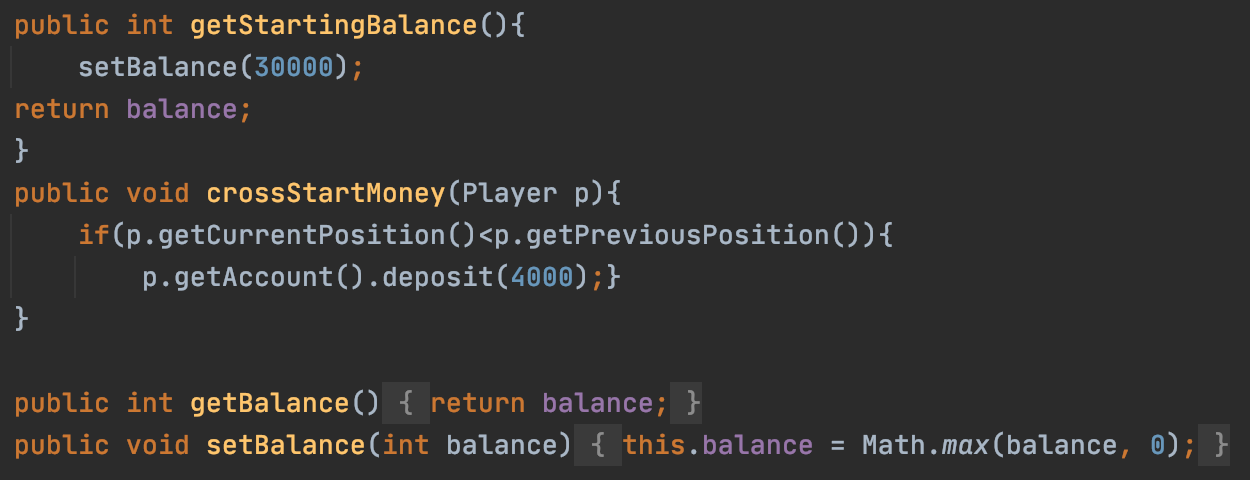
\includegraphics[width=\textwidth]{sources/7_implementering/Account GetSet.png}
    \caption{Account Getters & Setters}
    \label{fig:accGetSet}
\end{figure}
Sidst har vi get- og setBalance, som kan bruges til at få fat i en spillers account og ændre på det.

